\documentclass[english, 11 pt, class=article, crop=false]{standalone}
\usepackage[T1]{fontenc}
%\renewcommand*\familydefault{\sfdefault} % For dyslexia-friendly text
\usepackage{lmodern} % load a font with all the characters
\usepackage{geometry}
\geometry{verbose,paperwidth=16.1 cm, paperheight=24 cm, inner=2.3cm, outer=1.8 cm, bmargin=2cm, tmargin=1.8cm}
\setlength{\parindent}{0bp}
\usepackage{import}
\usepackage[subpreambles=false]{standalone}
\usepackage{amsmath}
\usepackage{amssymb}
\usepackage{esint}
\usepackage{babel}
\usepackage{tabu}
\makeatother
\makeatletter

\usepackage{titlesec}
\usepackage{ragged2e}
\RaggedRight
\raggedbottom
\frenchspacing

% Norwegian names of figures, chapters, parts and content
\addto\captionsenglish{\renewcommand{\figurename}{Figur}}
\makeatletter
\addto\captionsenglish{\renewcommand{\chaptername}{Kapittel}}
\addto\captionsenglish{\renewcommand{\partname}{Del}}


\usepackage{graphicx}
\usepackage{float}
\usepackage{subfig}
\usepackage{placeins}
\usepackage{cancel}
\usepackage{framed}
\usepackage{wrapfig}
\usepackage[subfigure]{tocloft}
\usepackage[font=footnotesize,labelfont=sl]{caption} % Figure caption
\usepackage{bm}
\usepackage[dvipsnames, table]{xcolor}
\definecolor{shadecolor}{rgb}{0.105469, 0.613281, 1}
\colorlet{shadecolor}{Emerald!15} 
\usepackage{icomma}
\makeatother
\usepackage[many]{tcolorbox}
\usepackage{multicol}
\usepackage{stackengine}

\usepackage{esvect} %For vectors with capital letters

% For tabular
\usepackage{array}
\usepackage{multirow}
\usepackage{longtable} %breakable table

% Ligningsreferanser
\usepackage{mathtools}
\mathtoolsset{showonlyrefs}

% index
\usepackage{imakeidx}
\makeindex[title=Indeks]

%Footnote:
\usepackage[bottom, hang, flushmargin]{footmisc}
\usepackage{perpage} 
\MakePerPage{footnote}
\addtolength{\footnotesep}{2mm}
\renewcommand{\thefootnote}{\arabic{footnote}}
\renewcommand\footnoterule{\rule{\linewidth}{0.4pt}}
\renewcommand{\thempfootnote}{\arabic{mpfootnote}}

%colors
\definecolor{c1}{cmyk}{0,0.5,1,0}
\definecolor{c2}{cmyk}{1,0.25,1,0}
\definecolor{n3}{cmyk}{1,0.,1,0}
\definecolor{neg}{cmyk}{1,0.,0.,0}

% Lister med bokstavar
\usepackage[inline]{enumitem}

\newcounter{rg}
\numberwithin{rg}{chapter}
\newcommand{\reg}[2][]{\begin{tcolorbox}[boxrule=0.3 mm,arc=0mm,colback=blue!3] {\refstepcounter{rg}\phantomsection \large \textbf{\therg \;#1} \vspace{5 pt}}\newline #2  \end{tcolorbox}\vspace{-5pt}}

\newcommand\alg[1]{\begin{align} #1 \end{align}}

\newcommand\eks[2][]{\begin{tcolorbox}[boxrule=0.3 mm,arc=0mm,enhanced jigsaw,breakable,colback=green!3] {\large \textbf{Eksempel #1} \vspace{5 pt}\\} #2 \end{tcolorbox}\vspace{-5pt} }

\newcommand{\st}[1]{\begin{tcolorbox}[boxrule=0.0 mm,arc=0mm,enhanced jigsaw,breakable,colback=yellow!12]{ #1} \end{tcolorbox}}

\newcommand{\spr}[1]{\begin{tcolorbox}[boxrule=0.3 mm,arc=0mm,enhanced jigsaw,breakable,colback=yellow!7] {\large \textbf{Språkboksen} \vspace{5 pt}\\} #1 \end{tcolorbox}\vspace{-5pt} }

\newcommand{\sym}[1]{\colorbox{blue!15}{#1}}

\newcommand{\info}[2]{\begin{tcolorbox}[boxrule=0.3 mm,arc=0mm,enhanced jigsaw,breakable,colback=cyan!6] {\large \textbf{#1} \vspace{5 pt}\\} #2 \end{tcolorbox}\vspace{-5pt} }

\newcommand\algv[1]{\vspace{-11 pt}\begin{align*} #1 \end{align*}}

\newcommand{\regv}{\vspace{5pt}}
\newcommand{\mer}{\textsl{Merk}: }
\newcommand{\mers}[1]{{\footnotesize \mer #1}}
\newcommand\vsk{\vspace{11pt}}
\newcommand\vs{\vspace{-11pt}}
\newcommand\vsb{\vspace{-16pt}}
\newcommand\sv{\vsk \textbf{Svar} \vspace{4 pt}\\}
\newcommand\br{\\[5 pt]}
\newcommand{\figp}[1]{../fig/#1}
\newcommand\algvv[1]{\vs\vs\begin{align*} #1 \end{align*}}
\newcommand{\y}[1]{$ {#1} $}
\newcommand{\os}{\\[5 pt]}
\newcommand{\prbxl}[2]{
\parbox[l][][l]{#1\linewidth}{#2
	}}
\newcommand{\prbxr}[2]{\parbox[r][][l]{#1\linewidth}{
		\setlength{\abovedisplayskip}{5pt}
		\setlength{\belowdisplayskip}{5pt}	
		\setlength{\abovedisplayshortskip}{0pt}
		\setlength{\belowdisplayshortskip}{0pt} 
		\begin{shaded}
			\footnotesize	#2 \end{shaded}}}

\renewcommand{\cfttoctitlefont}{\Large\bfseries}
\setlength{\cftaftertoctitleskip}{0 pt}
\setlength{\cftbeforetoctitleskip}{0 pt}

\newcommand{\bs}{\\[3pt]}
\newcommand{\vn}{\\[6pt]}
\newcommand{\fig}[1]{\begin{figure}
		\centering
		\includegraphics[]{\figp{#1}}
\end{figure}}

\newcommand{\figc}[2]{\begin{figure}
		\centering
		\includegraphics[]{\figp{#1}}
		\caption{#2}
\end{figure}}

\newcommand{\sectionbreak}{\clearpage} % New page on each section

\newcommand{\nn}[1]{
\begin{equation}
	#1
\end{equation}
}

% Equation comments
\newcommand{\cm}[1]{\llap{\color{blue} #1}}

\newcommand\fork[2]{\begin{tcolorbox}[boxrule=0.3 mm,arc=0mm,enhanced jigsaw,breakable,colback=yellow!7] {\large \textbf{#1 (forklaring)} \vspace{5 pt}\\} #2 \end{tcolorbox}\vspace{-5pt} }
 
%colors
\newcommand{\colr}[1]{{\color{red} #1}}
\newcommand{\colb}[1]{{\color{blue} #1}}
\newcommand{\colo}[1]{{\color{orange} #1}}
\newcommand{\colc}[1]{{\color{cyan} #1}}
\definecolor{projectgreen}{cmyk}{100,0,100,0}
\newcommand{\colg}[1]{{\color{projectgreen} #1}}

% Methods
\newcommand{\metode}[2]{
	\textsl{#1} \\[-8pt]
	\rule{#2}{0.75pt}
}

%Opg
\newcommand{\abc}[1]{
	\begin{enumerate}[label=\alph*),leftmargin=18pt]
		#1
	\end{enumerate}
}
\newcommand{\abcs}[2]{
	\begin{enumerate}[label=\alph*),start=#1,leftmargin=18pt]
		#2
	\end{enumerate}
}
\newcommand{\abcn}[1]{
	\begin{enumerate}[label=\arabic*),leftmargin=18pt]
		#1
	\end{enumerate}
}
\newcommand{\abch}[1]{
	\hspace{-2pt}	\begin{enumerate*}[label=\alph*), itemjoin=\hspace{1cm}]
		#1
	\end{enumerate*}
}
\newcommand{\abchs}[2]{
	\hspace{-2pt}	\begin{enumerate*}[label=\alph*), itemjoin=\hspace{1cm}, start=#1]
		#2
	\end{enumerate*}
}

% Oppgaver
\newcommand{\opgt}{\phantomsection \addcontentsline{toc}{section}{Oppgaver} \section*{Oppgaver for kapittel \thechapter}\vs \setcounter{section}{1}}
\newcounter{opg}
\numberwithin{opg}{section}
\newcommand{\op}[1]{\vspace{15pt} \refstepcounter{opg}\large \textbf{\color{blue}\theopg} \vspace{2 pt} \label{#1} \\}
\newcommand{\ekspop}[1]{\vsk\textbf{Gruble \thechapter.#1}\vspace{2 pt} \\}
\newcommand{\nes}{\stepcounter{section}
	\setcounter{opg}{0}}
\newcommand{\opr}[1]{\vspace{3pt}\textbf{\ref{#1}}}
\newcommand{\oeks}[1]{\begin{tcolorbox}[boxrule=0.3 mm,arc=0mm,colback=white]
		\textit{Eksempel: } #1	  
\end{tcolorbox}}
\newcommand\opgeks[2][]{\begin{tcolorbox}[boxrule=0.1 mm,arc=0mm,enhanced jigsaw,breakable,colback=white] {\footnotesize \textbf{Eksempel #1} \\} \footnotesize #2 \end{tcolorbox}\vspace{-5pt} }
\newcommand{\rknut}{
Rekn ut.
}

%License
\newcommand{\lic}{\textit{Matematikken sine byggesteinar by Sindre Sogge Heggen is licensed under CC BY-NC-SA 4.0. To view a copy of this license, visit\\ 
		\net{http://creativecommons.org/licenses/by-nc-sa/4.0/}{http://creativecommons.org/licenses/by-nc-sa/4.0/}}}

%referances
\newcommand{\net}[2]{{\color{blue}\href{#1}{#2}}}
\newcommand{\hrs}[2]{\hyperref[#1]{\color{blue}\textsl{#2 \ref*{#1}}}}
\newcommand{\rref}[1]{\hrs{#1}{regel}}
\newcommand{\refkap}[1]{\hrs{#1}{kapittel}}
\newcommand{\refsec}[1]{\hrs{#1}{seksjon}}

\newcommand{\mb}{\net{https://sindrsh.github.io/FirstPrinciplesOfMath/}{MB}}


%line to seperate examples
\newcommand{\linje}{\rule{\linewidth}{1pt} }

\usepackage{datetime2}
%%\usepackage{sansmathfonts} for dyslexia-friendly math
\usepackage[]{hyperref}


\newcommand{\note}{Merk}
\newcommand{\notesm}[1]{{\footnotesize \textsl{\note:} #1}}
\newcommand{\ekstitle}{Eksempel }
\newcommand{\sprtitle}{Språkboksen}
\newcommand{\expl}{forklaring}

\newcommand{\vedlegg}[1]{\refstepcounter{vedl}\section*{Vedlegg \thevedl: #1}  \setcounter{vedleq}{0}}

\newcommand\sv{\vsk \textbf{Svar} \vspace{4 pt}\\}

%references
\newcommand{\reftab}[1]{\hrs{#1}{tabell}}
\newcommand{\rref}[1]{\hrs{#1}{regel}}
\newcommand{\dref}[1]{\hrs{#1}{definisjon}}
\newcommand{\refkap}[1]{\hrs{#1}{kapittel}}
\newcommand{\refsec}[1]{\hrs{#1}{seksjon}}
\newcommand{\refdsec}[1]{\hrs{#1}{delseksjon}}
\newcommand{\refved}[1]{\hrs{#1}{vedlegg}}
\newcommand{\eksref}[1]{\textsl{#1}}
\newcommand\fref[2][]{\hyperref[#2]{\textsl{figur \ref*{#2}#1}}}
\newcommand{\refop}[1]{{\color{blue}Oppgave \ref{#1}}}
\newcommand{\refops}[1]{{\color{blue}oppgave \ref{#1}}}
\newcommand{\refgrubs}[1]{{\color{blue}gruble \ref{#1}}}

\newcommand{\openmathser}{\openmath\,-\,serien}

% Exercises
\newcommand{\opgt}{\newpage \phantomsection \addcontentsline{toc}{section}{Oppgaver} \section*{Oppgaver for kapittel \thechapter}\vs \setcounter{section}{1}}


% Sequences and series
\newcommand{\sumarrek}{Summen av en aritmetisk rekke}
\newcommand{\sumgerek}{Summen av en geometrisk rekke}
\newcommand{\regnregsum}{Regneregler for summetegnet}

% Trigonometry
\newcommand{\sincoskomb}{Sinus og cosinus kombinert}
\newcommand{\cosfunk}{Cosinusfunksjonen}
\newcommand{\trid}{Trigonometriske identiteter}
\newcommand{\deravtri}{Den deriverte av de trigonometriske funksjonene}
% Solutions manual
\newcommand{\selos}{Se løsningsforslag.}
\newcommand{\se}[1]{Se eksempel på side \pageref{#1}}

%Vectors
\newcommand{\parvek}{Parallelle vektorer}
\newcommand{\vekpro}{Vektorproduktet}
\newcommand{\vekproarvol}{Vektorproduktet som areal og volum}


% 3D geometries
\newcommand{\linrom}{Linje i rommet}
\newcommand{\avstplnpkt}{Avstand mellom punkt og plan}


% Integral
\newcommand{\bestminten}{Bestemt integral I}
\newcommand{\anfundteo}{Analysens fundamentalteorem}
\newcommand{\intuf}{Integralet av utvalge funksjoner}
\newcommand{\bytvar}{Bytte av variabel}
\newcommand{\intvol}{Integral som volum}
\newcommand{\andordlindif}{Andre ordens lineære differensialligninger}



\begin{document}
\section{GeoGebra}	
\subsection{CAS}	
\subsubsection{Definere variabler \label{defvar}}
Hvis vi ønsker å definere variabler som vi skal bruke i andre celler, må vi skrive \texttt{:=} . I figuren under er forskjellen mellom \texttt{=} og \texttt{:=} demonstrert med et forsøk på å finne $ f'(x) $ til funksjonen $ f(x)=x^2 $:
\begin{figure}
	\centering
	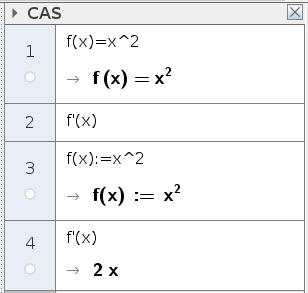
\includegraphics[scale=0.5]{fig/fder}
\end{figure}
Av figuren legger vi også merke til at celle 3 og celle 4 er markert med en hvit runding. Dette indikerer at størrelsen vil vises i \textsl{Grafikkfelt} eller \textsl{Grafikkfelt 3D} hvis man trykker på markøren (den skal da bli blå).
\subsubsection{Celle-referanser}

Ofte kommer vi ut for situasjoner der vi ønsker å bruke uttrykket vi har funnet i tidligere celler. Som eksempel har vi i celle 1 skrevet inn volumet $ v $ av en kule med radius $ r $, mens i celle 2 har vi volumet $ V $ av en kule med radius $ R $. Ønsker vi å finne forholdet mellom disse, kan vi bruke cellereferanser som hjelpemiddel. For å referere til celle 1 skriver vi \texttt{\$1} og for celle 2 skriver vi \texttt{\$2}. Forholdet $ \frac{v}{V} $ kan vi da skriver som \texttt{\$1/\$2}:
\begin{figure}
	\centering
	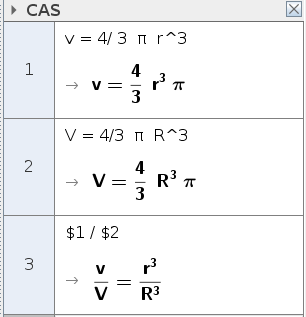
\includegraphics[scale=0.5]{fig/ref}
\end{figure}

\subsubsection{Lister}
Når et uttrykk står inni sløyfeparanteser \{\}, betyr det at det er laget en liste. En liste inneholder flere elementer som vi kan hente ut. Dette gjør vi ved å skrive paranteser bak listen, hvor vi angir nummeret til elementet i listen.
\begin{figure}
	\centering
	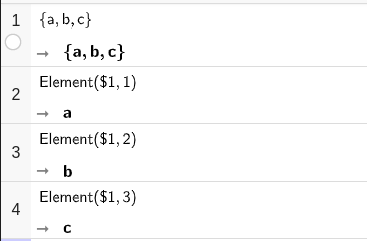
\includegraphics[scale=0.5]{fig/liste}
\end{figure}

Lister bruker vi også når vi skal løse liginger med flere ukjente:
\begin{figure}
	\centering
	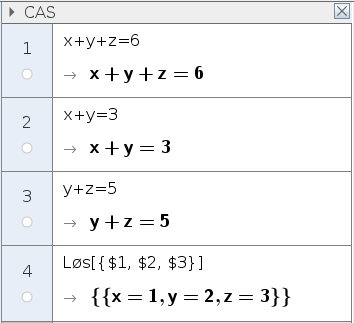
\includegraphics[scale=0.5]{fig/lign}
\end{figure}
\subsubsection{Høyre- og venstresiden \label{hogl}}
De fleste uttrykkene vi jobber med i CAS inneholder et $ = $ tegn. Disse uttrykkene er en ligning med en venstre- og høyreside. Ofte ønsker vi å bruke uttrykket på bare én av disse sidene, og oftest høyresiden. Som eksempel har vi løst ligningen $ (a+b)x = c $ og definert funksjonen $ f(x)= d x^2 $. Vi ønsker så å sette løsningen av ligningen inn i funksjonen. Dette gjør vi ved hjelp av \texttt{HøyreSide}-kommandoen (resulatet uten bruken av denne er vist i celle 4).
\begin{figure}
	\centering
	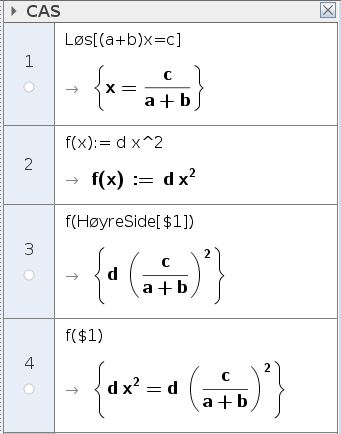
\includegraphics[scale=0.5]{fig/hoyre}
\end{figure}
\subsubsection{ByttUt}
Noen ganger ønsker vi å endre en variabel i et utrykk. For å gjøre dette kan vi anvende \texttt{{ByzttUt}{<Uttrykk>, <Liste med forandringer>}}. La oss se på uttrykket
\[ \frac{a+b}{c} \]
Vi ønsker nå å sette $ {a=d }$, $ {b=2} $ og $ {c=f} $. Dette kan vi gjør ved å skrive følgende:
\begin{figure}
	\centering
	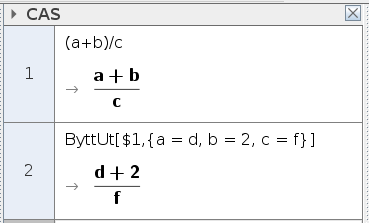
\includegraphics[scale=0.5]{fig/cas2}
\end{figure}	
\newpage
\subsection{Knapper og kommandoer}
\subsubsection*{Grafikkfelt}
Knappene velges fra rullemenyer på verktøylinjen. Nummereringen av menyene er fra venstre.\vsk

\begin{tabular}{@{}l}
	\,
\includegraphics[scale=0.4]{fig/pkt} Lager et nytt punkt. (Meny nr. 1) \\
	\,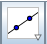
\includegraphics[scale=0.4]{fig/lin} Lager linje mellom to punkt. (Meny nr. 2)\\	
	\,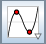
\includegraphics[scale=0.4]{fig/ekst} Finner topp- og bunnpunkt til en funksjon. (Meny nr. 2)\\
	\,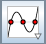
\includegraphics[scale=0.4]{fig/nul} Finner nullpunktene til en funksjon. (Meny nr. 2)	\\
	\,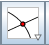
\includegraphics[scale=0.4]{fig/skj} Finner skjæringspunkt mellom to objekt. (Meny nr. 3)\\	
	\,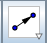
\includegraphics[scale=0.4]{fig/vek} Lager vektoren mellom to punkt (Meny nr. 3)\\		
	\,
\includegraphics[scale=0.4]{fig/tekst} Lager en tekstboks. (Meny nr. 10)\\		
	\,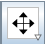
\includegraphics[scale=0.4]{fig/flytt} Flytter grafikkfeltet. Endrer verdiavstanden hvis man peker på aksene. \\
	\hspace{1cm}(Meny nr. 10)\\			
\end{tabular}
\subsubsection*{CAS}
\begin{tabular}{@{}l}
	\;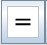
\includegraphics[scale=0.4]{fig/erlik} Gjengir uttrykket som er inntastet, ofte i forkortet form.\\	
	\;
\includegraphics[scale=0.4]{fig/brin} Gjengir uttrykket som er inntastet.\\	
	\;
\includegraphics[scale=0.4]{fig/caerlik} Gir tilnærmet verdi av et uttrykk (som desimaltall). \\	
	\;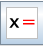
\includegraphics[scale=0.4]{fig/x} Gir eksaktløsningen av en ligning.\\
	\;
\includegraphics[scale=0.4]{fig/xca} Gir tilnærmet løsning av en ligning som desimaltall.\\
	
\end{tabular}

\subsubsection{Hurtigtaster}
\begin{tabular}{@{}c | c |c | c }
	&\textbf{Beskrivelse} & \textbf{PC }& \textbf{Mac} \\ \hline
	$ \sqrt{} $	& kvadratrot& \texttt{alt\,+\,r} &\texttt{alt\,+\,r} \\\hline
	$ \pi $	& pi& \texttt{alt\,+\,p} & \texttt{alt\,+\,p}\\\hline
	$ \infty $ &uendelig& \texttt{alt\,+\,u} &\texttt{alt\,+\,,}  \\\hline
	$ \otimes $&kryssprodukt & \texttt{alt\,+\,shift\,+\,8}&\texttt{ctrl\,+\,shift\,+\,8} \\\hline
	$ e $&eulers tall & \texttt{alt\,+\,e}& \texttt{alt\,+\,e}\\\hline
	$ {}^\circ $&gradtegnet ($ \frac{\pi}{180} $) & \texttt{alt\,+\,o}& \texttt{alt\,+\,o}
	\\\hline	
\end{tabular}
\newpage
\label{commandliststart}
\subsubsection{Kommandoliste}
\begin{itemize}
\item \cmds{abs( <x> )}
{Finner lengden til et objekt \textit{x}.
}

\item \cmds{acos( <x> )}
{
I algebrafelt: Gir vinkelen på intervallet $ [0^\circ, 180^\circ] $ som har cosinus-verdi $ x $. \os
I CAS: Gir vinkelen på intervallet $ [0, \pi] $ som har cosinus-verdi $ x $.
}

\item \cmds{asin( <x> )}
{
I algebrafelt: Gir vinkelen på intervallet $ [-90^\circ, 90^\circ] $ som har sinus-verdi $ x $.\os

I CAS: Gir vinkelen på intervallet $ [-\frac{\pi}{2}, \frac{\pi}{2}] $ som har sinus-verdi $ x $.
}

\item \cmds{atan( <x> )}
{
I algebrafelt: Gir vinkelen på intervallet $ [-90^\circ, 90^\circ] $ som har tangens-verdi $ x $.\os

I CAS: Gir vinkelen på intervallet $ [-\frac{\pi}{2}, \frac{\pi}{2}] $ som har sinus-verdi $ x $.
}

\item \cmds{Asymptote( <Funksjon> )}
{Finner asymptotene til en funksjon.}



\item \cmds{Avstand( <Punkt>, <Objekt> )}
{Gir avstanden fra et punkt til et objekt.}

\item \cmds{ByttUt( <Uttrykk>, <Liste med forandringer> ) }
{Viser et gitt uttrykk etter endring av variabler, gitt i en liste.}

\item \cmds{Deriverte( <Funksjon> )}{Gir den deriverte av en funksjon.\\	
	\mers{
		For en definert funksjon $ f(x) $, kan man like gjerne skrive \texttt{f'(x)}.
}}

\item \cmds{Ekstremalpunkt( <Funksjon>, <Start>, <Slutt> )}{Finner lokale ekstremalpunkt og ekstremalverdier for en funksjon $ f $ på et gitt intervall.}

\item \cmds{Ekstremalpunkt( <Polynom> )}
{Finner lokale ekstremalpunkt og ekstremalverdier til et polynom.}

\item \cmds{Funksjon ( <Funksjon>, <Start>, <Slutt> )}
{Tegner en funksjon på et gitt intervall.}

\newpage
\item \cmds{Høyde( <Objekt> )}
{Gir avstanden fra toppunkt til grunnflate i et objekt.\\ 
	\mers{Avstanden har retning, og derfor kan den noen ganger være negativ. Tallverdien er den geometriske høyden.}}

\item \cmds{HøyreSide ( <Likning> )}
{Gir høyresiden til en likning.}

\item \cmds{HøyreSide ( <Liste med likninger> )}
{Gir en liste med høyresidene i en liste med ligninger.}

\item \cmds{Integral ( <Funksjon> )}
{Gir uttrykket til det ubestemte integralet av en funksjon. \\
\mers{Hvis kommandoen skrives i inntastingsfeltet, blir konstantleddet utelatt}
}

\item \cmds{Integral( <Funksjon>, <Start>, <Slutt> )}
{Gir det bestemte integralet av en funksjon på et intervall.}

\item \cmds{Integral( <Variabel> )}
{Gir uttrykket til det ubestemte integralet til en funksjon av gitt variabel. (Brukes dersom man ønsker å integrere funksjoner avhengig av en annen variabel enn $ x $).}

\item \cmds{Kule( <Punkt>, <Radius> )}
{Viser en kule i Grafikkfelt 3D med sentrum i et gitt punkt og med en gitt radius.}

\item \cmds{Kurve( <Uttrykk>, <Uttrykk>, <Uttrykk>, <Parametervariabel>, <Start>, <Slutt> )}
{Viser parameteriseringen av en kurve i Grafikkfelt 3D på et gitt intervall. Uttrykkene er henholdsvis uttrykkene for $ {x, y} $ og $ z $-koordinatene, bestemt av en gitt parametervariabel. \\
\mers{
	Med mindre et bestemt intervall av kurven er ønsket, er det bedre å skrive parameteriseringen direkte inn i inntastingsfeltet som \texttt{A+t*u}, hvor $ A $ er et punkt på linja og $ u$ er en retningsvektor.
}}	

\item \cmds{Linje ( <Punkt>, <Punkt> )}{ Gir uttrykket til en linje mellom to punkt. Hvis punktene har tre koordinater besår uttrykket av et punkt på linja og en fri variabel $ \lambda $ mulitplisert med en retningsvektor.}	

\item \cmds{Løs ( <Likning med x> )}{
	Løser en likning med $ x $ som ukjent.
}

\item 
\cmds{Løs( <Liste med likninger>, <Liste med variabler> )}
{Finner alle løsninger av en liste med ligninger med gitte variabel som ukjente.}

\item \cmds{Løs( <Likning>, <Variabel> )}
{Finner alle løsninger av en gitt likning med en gitt variabel som ukjent.}

\item \cmds{Maks( <Funksjon>, <Start x-verdi>, <Slutt x-verdi> )}{Finner absolutt maksimum og maskimalpunkt for en funksjon $ f $ på et gitt intervall.}

\item \cmds{Min}( <Funksjon>, <Start x-verdi>, <Slutt x-verdi> ) {Finner absolutt minimum og minimumspunkt for en funksjon $ f $ på et gitt intervall.}

\item \cmds{Nullpunkt( <Polynom> )}
{Finner alle nullpunkter til et polynom.}

\item \cmds{NullpunktIntervall( <Funksjon>, <Start>, <Slutt> )}
{Finner alle nullpunkter på et gitt intervall til en hvilken som helst funksjon.}

\item \cmds{Plan( <Punkt>, <Punkt>, <Punkt> )}
{Viser et plan i Grafikkfelt 3D, utspent av to av vektorene mellom tre gitte punkt.}

\item \cmds{Prisme( <Punkt>, <Punkt>, ... )}
{Framstiller en prisme i Grafikkfelt 3D. {\tt Prisme[A,B,C,D]} lager en prisme med grunnflate $ ABC $ og tak $ DEF $, {\tt Prisme[A,B,C,D,E]} har grunnflate $ ABCD $ og tak $ EFG $. $ F, G$ og eventelt $ E $ blir konstruert av GeoGebra slik at hver sideflate er et parallellogram. Under kategorien \textsl{Prisme} i algebrafaltet finner man en konstant som oppgir volumet til pyramiden.}

\item \cmds{Punkt( <Liste> )}{Lager et punkt med koordinater gitt som liste. \\
	
	\mers{For å lage punktet $ (x, y) $, kan man liksågodt skrive \texttt{(x,y)} i inntastingsfeltet. Skriver man \texttt{(x,y)} i CAS lager man vektoren $ [x, y] $.}
}

\item \cmds{Pyramide( <Punkt>, <Punkt>, ... )}
{Framstiller en pyramide i Grafikkfelt 3D. {\tt Pyramide[A,B,C,D]} lager en pyramide med grunnflate ${ A, B, C} $ og toppunkt $ D $, mens {\tt Pyramide[A,B,C,D, E]} har grunnflate ${ A, B, C, D }$ og toppunkt $ E $. Under kategorien \textsl{Pyramide} i algebrafaltet finner man en konstant som oppgir volumet til pyramiden.}

\item \cmds{RegLin( <Liste> )}
{Bruker regresjon med en rett linje for å tilpasse punkt gitt i en liste.}

\item \cmds{RegEksp( <Liste> )}
{Bruker regresjon med en eksponentialfunksjon for å tilpasse punkt gitt i en liste.}

\item \cmds{RegPoly( <Liste>, <Grad> )}
{Bruker regresjon med et polynom av gitt grad for å tilpasse punkt gitt i en liste.}

\item \cmds{RegPot( <Liste> )}
{Bruker regresjon med en potensfunksjon for å tilpasse punkt gitt i en liste.}

\item \cmds{RegSin( <Liste> )}
{Bruker regresjon med en sinusfunksjon for å tilpasse punkt gitt i en liste.	}

\item \cmds{Skalarprodukt( <Vektor>, <Vektor> )} 
{Finner skalarproduktet av to vektorer. \\
\mers{For to vektorer $u$ og $v$ kan man like gjerne skrive \texttt{u*v}.}}

\item \cmds{Skjæring( <Objekt>, <Objekt> )}
{Finner skjæringspunktene mellom to objekter. 
}

\item \cmds{Skjæring( <Funksjon>, <Funksjon>, <Start>, <Slutt> )}
{Finner skjæringspunktene mellom to funksjoner på et gitt intervall.}

\item \cmds{Sum( <Uttrykk>, <Variabel>, <Start>, <Slutt> )}{
	Finner summen av en rekke med en løpende variabel på et intervall.
}

\item \cmds{TrigKombiner( <Funksjon> )}
{Skriver om et uttrykk på formen $ a\sin (kx) + b\cos (kx) $ til et kombinert uttrykk på formen $ r\cos (kx-c) $.}

\item \cmds{TrigKombiner( <Funksjon>, sin(x) )}{Skriver om en funksjon på formen $ {a\sin (kx) + b\cos (kx) }$ til et kombinert uttrykk på formen $ r\sin (kx+c) $.}

\item \cmds{Vektor( <Punkt> )}{
	Lager vektoren fra origo til et gitt punkt. \\
	\mers{I CAS kan man lage vektoren $ {[x, y]} $ ved å skrive \texttt{(x,y)}, dette anbefales.}
}

\item \cmds{Vektorprodukt( <Vektor>, <Vektor> )}{Finner vektorproduktet av to vektorer. \\
	\mers{For to vektorer $u$ og $v$ kan man like gjerne skrive \texttt{u}$ \otimes $\texttt{v}. }
}

\item \cmds{Vendepunkt( <Polynom> )}
{Finner vendepunktene til et polynom.}

\item \cmds{VenstreSide( <Likning> )}
{Gir venstresiden til en likning.}

\item \cmds{VenstreSide( <Liste med likninger> )}
{Gir en liste med venstresidene i en liste med ligninger.}

\item \cmds{Vinkel( <Vektor>, <Vektor> )}
{Gir vinkelen mellom to vektorer. Kan også brukes for vinkel mellom plan/linjer, plan/plan og linje/linje}
\end{itemize}
\label{commandlistend}


\end{document}






\regsin

\retn

\skalar



\summ



\trikomb

\vektor

\vekpro

\vend

